\documentclass{report}
\usepackage{graphicx}
\usepackage{float}
\usepackage{amsmath}
\usepackage{amsthm}
\usepackage{caption}
\usepackage{algorithm}
\usepackage{hyperref}
\usepackage{listingsutf8}
\usepackage[noend]{algpseudocode}
\usepackage[a4paper]{geometry}

\renewcommand{\algorithmicrequire}{\textbf{Input:}}
\renewcommand{\algorithmicensure}{\textbf{Output:}}

\usepackage{mathtools}
\DeclarePairedDelimiter\ceil{\lceil}{\rceil}

\def \scalingfactor{.8}

\begin{document}

\title{Studying the Fermi architecture to improve the Integer capabilities for cryptology}
\author{Cl\'{e}ment Humbert, Tristan Overney\and Paolo Ienne, Andrea Miele, Ewaida Mohsen (Supervisors)}
\date{\today}
\maketitle

\nocite{*}

\setcounter{tocdepth}{1}
\tableofcontents
\listoffigures

\chapter{Introduction}

    Due to their computing power, GPUs have been used in different scientific fields to perform
    non-graphical computations for a while. They are used for particle and molecular dynamic 
    modeling, astrophysics and fluid mechanic modeling.
    More recently they've been used to investigate the possibility of assessing the security of
    cryptographic applications, in particular RSA and elliptic curves encryption~\cite{cofact14}.
    Cryptology-related applications make heavy use of very large integer operations.
    Here's a building block of the algorithms used~\cite{cofact14}:
    \begin{algorithm}
    \caption{Large operands multiplication}\label{alg:mulalgo}
    \begin{algorithmic}[1]
        \Require{Integers x and $Y=\sum_{i=0}^{n-1}Y_ir^i$ such that $0\leq x$, $Y_i<r$ for $0\leq i<n$.}
        \Ensure{$Z=x\cdot Y = \sum_{i=0}^nZ_ir^i$}
        \State mul.lo($Z_0$, x, $Y_0$)
        \State mul.hi($Z_1$, x, $Y_0$)
        \State mad.lo.cc($Z_1$, x, $Y_1$, $Z_1$)
        \State mul.hi($Z_2$, x, $Y_1$)
        \For{$i=2$ to $n-2$}
            \State madc.lo.cc($Z_i$, x, $Y_i$, $Z_i$)
            \State mul.hi($Z_{i+1}$, x, $Y_i$)
        \EndFor
        \State madc.lo.cc($Z_{n-1}$, x, $Y_{n-1}$, $Z_{n-1}$)
        \State madc.hi($Z_n$, x, $Y_{n-1}$, 0)
        \State \textbf{return} $Z (=\sum_{i=0}^nZ_ir^i)$
    \end{algorithmic}
    \end{algorithm}

    Due to the nature of asymmetric cryptography, these applications are bound by
    integer computing capacity which is not the focus of GPU. GPUs are designed
    around floating-point number operations, for older GPUs it was single-precision
    floating-point number (which will be referred to as float from now on) operations and
    on more recent GPUs tendency is to focus on double precision floating-point number operations.
    Fermi generation is the last generation to have good integer multiplication performances
    compared to its float performance. It is one of the reasons it was chosen for this project.

\section{Goals}
    The aim of this project is to identify the limitations of Fermi GPUs
    when used for cryptology and applications using large integers arithmetic in order to suggest
    hardware changes accordingly.

\chapter{First approach}
    The first idea to enhance the cryptographic capabilities of the Fermi GPU was to
    build crypto specific hardware into the original hardware to expose new 
    operations (in the form of assembly opcodes) to the developers with the 
    shortest possible latency. 
    
    Montgomery multiplication, a special kind of modular multiplication, is an algorithm that is constantly used
    in cryptology; implementing it in hardware can be done in many ways.
    One of the most efficient way is the rolled implementation described by Algorithm~\ref{alg:montgomery}. Its operands $X$ and $Y$ are already prepared in software for the Montgomery multiplication.
    Algorithm~\ref{alg:montgomery} should be unrolled for the hardware implementation thus allowing to pipeline it.
    
    \begin{algorithm}
    \caption{Hardware Montgomery multiplier~\cite{montgomeryHard}}\label{alg:montgomery}
    \begin{algorithmic}[1]
        \Require{Integers $X$, $Y$ and $M$ with $0\leq X$, $Y < M$.}
        \Ensure{$P=(X * Y (2^n)^{-1})\text{ mod }M$.}
        \Statex $n$ is the number of bits in $X$.
        \Statex $x_i$ is the $i^{th}$ bit of $X$.
        \Statex $s_0$ is the least significant bit of $S$. 		
        \State $S := 0$; $C := 0$; \Comment $S$ is the Sum and $C$ is the carry
        \For{$i=0$; $i < n$; $i++$}
            \State $S,C := S + C + x_i * Y$; \Comment $S,C := ...$ is a carry-save adder assignation
            \State $S,C := S + C + s_0 * M$;
            \State $S := S$ div $2$; $C := C$ div $2$;  
        \EndFor
        \State $P := S + C$;
        \If{ $P \geq M$}
            \State $P := P - M$;
        \EndIf
        \State \textbf{return} $P$;
    \end{algorithmic}
    \end{algorithm}
    
    Another way to enhance cryptology performances is to have part of such
    an algorithm implemented in hardware, such as multiplications
    of numbers larger than 32bits, and the rest in software.
    

    The impact of the new opcodes were to be measured with the assistance of
    GPGPU-Sim~\cite{gpgpusim09} a Fermi architecture simulator. It was determined
    that new opcodes can be added to GPGPU-Sim and included in an instruction group
    to modify its latency (an unused operation could have been chosen to set the new
    instruction's latency).

    To determine the speed/size of the new components, the original cores have to
    be studied, as not much is known from Nvidia sources. Due to the lack of information
    this first approach was put aside and to understand 
    the cores structure and be able to suggest meaningful changes, a series of microbenchmarking 
    experiments had to be done. 

\chapter{Fermi's architecture}
    Before diving into the experiments and their results here's a quick-start
    guide to Nvidia's Fermi architecture and its vocabulary:
    \section{Streaming Multiprocessors}
    The largest building block inside the Fermi architecture is the 
    \emph{Streaming multiprocessor} (Figure~\ref{fig:SM} on page~\pageref{fig:SM})
    abbreviated SM in this report.
    \begin{figure}[H]
    \centering
        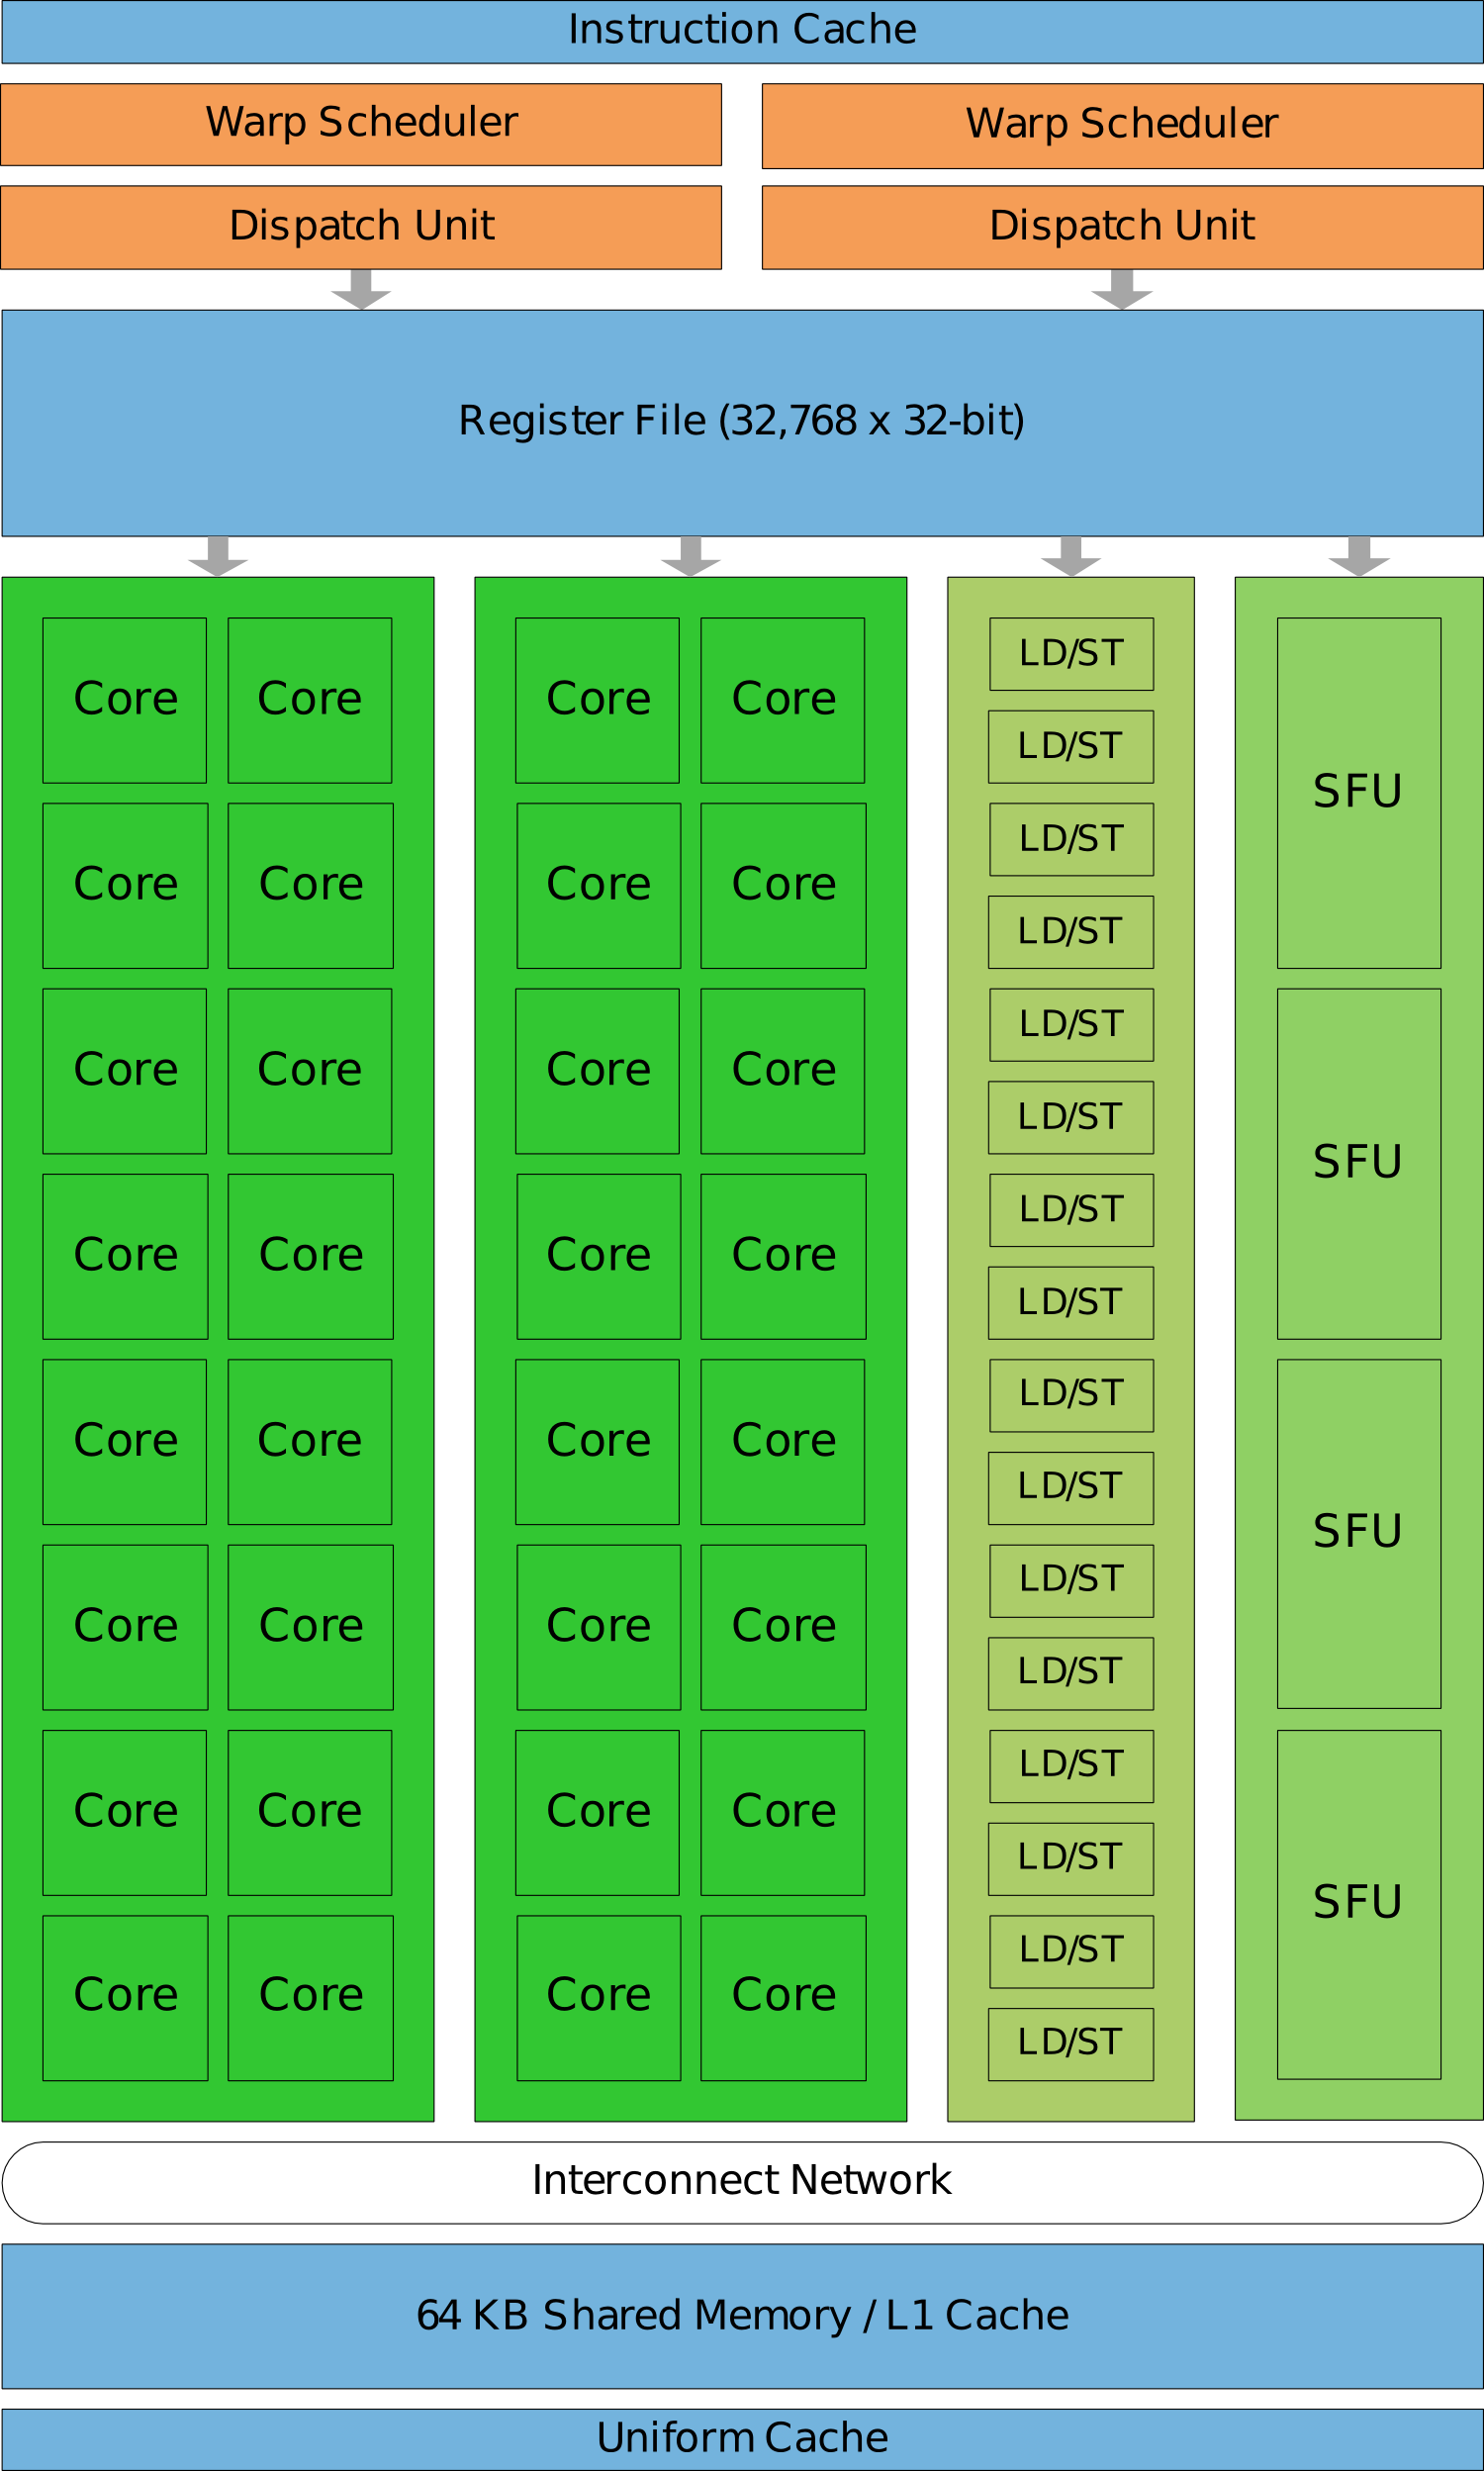
\includegraphics[width=0.75\linewidth]{pictures/Fermi}
        \captionsetup{justification=centering}
        \caption{Fermi's SM schematic representation~\cite{fermiwhitepap}.}
        \label{fig:SM}
    \end{figure}

    Each SM is composed of the following computation blocks~\cite{fermiwhitepap}:
    \begin{itemize}
        \item 32 CUDA cores in two groups of 16,
        \item 16 load/store units (LD/ST on the figure),
        \item 4 Special Functions Units (SFUs) dedicated to more complex
              arithmetic functions such as sines and logarithms.
    \end{itemize}
    
    As the SFU is dedicated to complex float operations, it can be replaced by integer computation components,
    thus it does not require any further research in this project. The focus of the experiments are the CUDA cores.

    \section{CUDA Cores}
    Figure~\ref{fig:CUDACore} represents a CUDA core according to Nvidia~\cite{fermiwhitepap}.
    
    \begin{figure}[H]
    \centering
        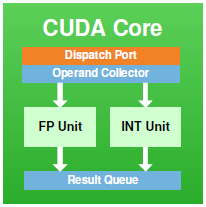
\includegraphics[width=0.5\linewidth]{pictures/CUDACore}
        \captionsetup{justification=centering}
        \caption{Schematic representation of Nvidia's CUDA Core.}
        \label{fig:CUDACore}
    \end{figure}
    
    From Figure~\ref{fig:CUDACore} the notion of twice 16 cores can be
    adjusted to 2x16 integers ALUs and 2x16 float ALUs. Integer is supported with at most 32-bits in Fermi.

    \section{Basics of Fermi's scheduling}
        \subsection{Grids and blocks} 
        A CUDA kernel (i.e.: a section of code that will run on the GPU) is
        launched with two parameters, a grid size and a block size. The grid 
        size is used to determine the number of SM on which the code will run.
        The block size determines how many threads will run the code inside each
        SM~\cite{cudaprog}. As the interesting properties are those of a single SM or even single
        core, every benchmarking experiment was done using a grid size of 1.

        \subsection{Warps}
        The second important scheduling unit is the warp. A warp consists
        of 32 threads. During each scheduling cycle, the scheduler selects two
        warps, for each of these it schedules 16 threads (making it 32
        threads scheduled, coming from two warps)~\cite{cudaprog}.

\chapter{Benchmarking}

\section{Methods}
	To get information about the microarchitecture of the CUDA cores, a series 
    of specially crafted CUDA kernels were used. These usually contain large 
    batches of instructions that were timed using the \texttt{clock64()} 
    function offered by the CUDA API.

	The benchmark programs have been run on a machine equipped with an Nvidia
    GeForce GTX 580 GPU used by Miele et al.~\cite{cofact14}.

\section{Pipeline properties}
	This section contains the results obtained through the previously described
	methods using large batches of integer multiplications.

	\subsection{Benchmark running times against number of threads}
	\label{par:pipeline_exp}
	\subsubsection{Description of the experiment}
	The first experiment aims at outlining the relation between the running
    times of the benchmark program and the number of threads running in parallel in
    a single block (the threads reside on one SM).
	\subsubsection{Expectations}
    Integer multiplications overall performances are expected to be worse than float multiplication as indicated
    in~\cite{cudaprog}. The reason for it is what these experiments are trying to discover.
    
	\subsubsection{Results and analysis}
    \begin{figure}[H]
    	\centering
	    \includegraphics[width=\scalingfactor\linewidth]{"graphics/float_vs_int_running_times"}
		\vspace{-15pt}
		\captionsetup{justification=centering}
        \caption{Running times of benchmark (in cycles) against number of threads.}
        \label{fig:int_fp_comp}
    \end{figure}
	
    Figure~\ref{fig:int_fp_comp} depicts the results of the first experiment,
    and shows that the integer multiplication times start to grow at 289 threads in the block against
    577 for the float multiplications.
   
    The flat line of integer and float multiplication are superposed up to 288 threads, meaning that
    either both multiplication have the same latency or they're latencies are hidden by a pipeline.
    The flat line for the floating point pipeline would mean that up to 576 threads the pipeline is not filled.
    Since an SM has 32 cores, we compute the pipeline depth as $\cfrac{576}{32} = 18$  stages. 
    This hypothesis seems to correlate with the running times of the integers multiplication. 
    
    Figure~\ref{fig:fp_prediction_512}
    represents the hypothesis made about the pipeline depth when 576 threads are running, $C_1$ to
    $C_{32}$ are the core of the single SM on which the experiment has been run. (1 to 16 is the
    first core group and 17 to 32 is the second one.) $t_{j,k}$ is the $k^{\text{th}}$ instruction of thread $j$. 
        \begin{figure}[H]
      \centering
       \begin{tabular}{ | r || c | c | c | c || c | c | c | }
    	    \hline
    	    time since beginning & $C_1$ & $C_2$ & ... & $C_{16}$ & $C_{17}$ & ... & $C_{32}$ \\ \hline  \hline
    	   1 & $t_{0,0}$ & $t_{1,0}$ & ... & $t_{15,0}$ & $t_{32, 0}$ & ... & $t_{47, 0}$ \\ \hline 
    	   2 & $t_{16,0}$ & $t_{17,0}$ & ... & $t_{31,0}$ & $t_{48, 0}$ & ... & $t_{63, 0}$ \\ \hline
    	   3 & $t_{64,0}$ & $t_{65,0}$ & ... & $t_{79,0}$ & $t_{96, 0}$ & ... & $t_{111, 0}$ \\ \hline
    	   ... & ... & ... & ... & ... & ... & ... & ... \\ \hline
    	   18 & $t_{528,0}$ & $t_{529,0}$ & ... & $t_{543,0}$ & $t_{560,0}$ & ... & $t_{575, 0}$ \\ \hline
    	   19 & $t_{0,1}$ & $t_{1,1}$ & ... & $t_{15,1}$ & $t_{32, 1}$ & ... & $t_{47, 1}$ \\ \hline
    	   ... & ... & ... & ... & ... & ... & ... & ... \\ \hline
  	\end{tabular}
  	\captionsetup{justification=centering}
  	\caption{Hypothesized running scheme for 576 threads with float multiplication.}
  	\label{fig:fp_prediction_512}
   \end{figure}
   
    On the other hand, the flat line of the integer experiment ends on 288 threads.
    Assuming a similar pipeline depth for the integer unit (18 stages) then we conclude that
    $\cfrac{288}{18} = 16$ cores only support integer multiplication.
   
    Figure~\ref{fig:int_prediction_256} represents the hypothesis made about the pipeline when 288
    threads are running, $C_1$ to $C_{32}$ are the core of the single SM on which the experiment
    has been run. (1 to 16 is the first core group and 17 to 32 is the second one.). The first
    core group is provided in integer multiplication but the second. $t_{j,k}$ is the $k^{\text{th}}$ instruction of thread $j$.
   \begin{figure}[H]
      \centering
       \begin{tabular}{ | r || c | c | c | c || c | c | c | }
    	    \hline
    	    time since beginning & $C_1$ & $C_2$ & ... & $C_{16}$ & $C_{17}$ & ... & $C_{32}$ \\ \hline  \hline
    	   1 & $t_{0,0}$ & $t_{1,0}$ & ... & $t_{15,0}$ & - & ... & - \\ \hline 
    	   2 & $t_{16,0}$ & $t_{17,0}$ & ... & $t_{31,0}$ & - & ... & - \\ \hline
    	   3 & $t_{32,0}$ & $t_{33,0}$ & ... & $t_{47,0}$ & - & ... & - \\ \hline
    	   ... & ... & ... & ... & ... & ... & ... & ... \\ \hline
    	   18 & $t_{272,0}$ & $t_{273,0}$ & ... & $t_{287,0}$ & - & ... & - \\ \hline
    	   19 & $t_{0,1}$ & $t_{1,1}$ & ... & $t_{15,1}$ & - & ... & - \\ \hline
    	   ... & ... & ... & ... & ... & ... & ... & ... \\ \hline
  	\end{tabular}
  	\captionsetup{justification=centering}
  	\caption{Hypothesized running scheme for 288 threads with integer number multiplication.}
  	\label{fig:int_prediction_256}
   \end{figure}

    To understand these deterioration points the next experiment has been designed.

\section{Understanding pipeline length and performance deterioration}
    \subsection{The experiment}
    With the results of \ref{par:pipeline_exp} in mind, it's clear that the pipelines depth 
    must be 18. The goal of the following experiment is to determine the cost of
    the loop used in the benchmarks to adjust the running times found and see if they match with
    the hypothesis about pipeline length and scheduling. 
	\subsubsection{Expectations}
	As seen in \ref{par:pipeline_exp} the cost of float
    operations goes up at 576 threads. This would imply that every pipeline of
    the SM is perfectly filled with 576 threads. Dividing 576 threads by
    the 32 cores gives a pipeline length of 18. In addition, the cost increase
    is suspected to be $1/9^\text{th}$ of the base cost as the scheduling is expected to be
    something like described in Table~\ref{fig:fp_prediction_513}.
    
    \begin{figure}[H]
      \centering
       \begin{tabular}{ | r || c | c | c | c || c | c | c | }
    	    \hline
    	    time since beginning & $C_1$ & $C_2$ & ... & $C_{16}$ & $C_{17}$ & ... & $C_{32}$ \\ \hline  \hline
    	   1 & $t_{0,0}$ & $t_{1,0}$ & ... & $t_{15,0}$ & $t_{32, 0}$ & ... & $t_{47, 0}$ \\ \hline 
    	   2 & $t_{16,0}$ & $t_{17,0}$ & ... & $t_{31,0}$ & $t_{48, 0}$ & ... & $t_{63, 0}$ \\ \hline
    	   3 & $t_{64,0}$ & $t_{65,0}$ & ... & $t_{79,0}$ & $t_{96, 0}$ & ... & $t_{111, 0}$ \\ \hline
    	   ... & ... & ... & ... & ... & ... & ... & ... \\ \hline
    	   18 & $t_{528,0}$ & $t_{529,0}$ & ... & $t_{543,0}$ & $t_{560,0}$ & ... & $t_{575, 0}$ \\ \hline
    	   19 & $t_{576,0}$ & - & ... & - & - & ... & - \\ \hline
    	   20 & - & - & ... & - & - & ... & - \\ \hline
    	   21 & $t_{0,1}$ & $t_{1,1}$ & ... & $t_{15,1}$ & $t_{32,1}$ & ... & $t_{47,1}$ \\ \hline
    	   ... & ... & ... & ... & ... & ... & ... & ... \\ \hline
  	\end{tabular}
  	\captionsetup{justification=centering}
  	\caption{Hypothesized running scheme for 577 threads with float multiplication.}
  	\label{fig:fp_prediction_513}
   \end{figure}

    The $\cfrac{1}{9}$ can be derived from the following formula
    \[ \cfrac{t_{\text{577threads}} - t_{\text{576threads}}}{t_{\text{576threads}}} \text{  .}\]
    The latency of an instruction is equal to the pipeline length, plus $\cfrac{1}{18}$ of
    it for every additional warp after the $18^{\text{th}}$. Thus, the latency $l$ of an 
    operation is $L + \text{max}\left(0, \left\lceil{\cfrac{N}{32} -18}\right\rceil\right)$ and to get the total
    running time of a benchmark, this latency must be added as a constant to
    represent the time the last instruction takes to get through the pipeline.

    The expansion of the previous formula gives
    \[ \cfrac{(18\cdot l_{576} + l_{577} + l_{577}) - (18\cdot l_{576} + l_{576})}{18\cdot l_{576} + l_{576}} \text{  .}\]
    This, with numerical values and simplifications is
    \[ \cfrac{(18\cdot 19 + 2\cdot 19) - (18^2 + 18)}{18^2 + 18} = \cfrac{1}{9}\text{  .}\] 

    To make sure the previous computations are not biased by the loop cost that is measured, the 
    million of operation was broken down into $10\cdot100,000$ operations and $1000\cdot1000$ operations.
    The difference would expose the cost of the for loop if it's significant.

	\subsubsection{Results and analysis}
    \begin{figure}[H]
		\centering
    			\includegraphics[width=\scalingfactor\linewidth]{"graphics/for-sizes-superpositions"}
		\vspace{-15pt}
		\captionsetup{justification=centering}
		\caption{Running a million operations broken down in 10 and 1000 loop iterations.}
        \label{fig:for-cost}
	\end{figure}
    
    Figure~\ref{fig:for-cost} suggests that only a insignificant amount of time is spent by the loop
    iterations' instructions.

\section{Mixing float and integer multiplication}
	\subsection{The experiment}
	The results of \ref{par:pipeline_exp} seem to point out that the number of 
    integer multiplications able to run in parallel on an SM is only half the number of 
    float multiplications. Leading to the conclusion that only one of
    the two 16 core groups of an SM was equipped with integer. These experiments issue 
    integer multiplications in parallel to float multiplications to confirm this hypothesis.
	\subsection{Benchmark running times, 1 float multiplication for 1 integer multiplication}
	If indeed only 1 out of 2 cores group can run integer multiplications,
    adding the same amount of float multiplications as there were integer
    multiplications should not increase the total time spent executing the benchmark 
    program as the float multiplications can
    be run on the other core group (the one that does not possess integer multipliers).
	
	One million multiplications of each kind have been run on 1 to 1024 threads to
    see if the results were comparable to the integer multiplications only graph (Figure~\ref{fig:int_fp_comp}).
	\begin{figure}[H]
		\centering
    			\includegraphics[width=\scalingfactor\linewidth]{"graphics/running_times_ratio11"}
		\vspace{-15pt}
		\captionsetup{justification=centering}
		\caption{Integer/Float multiplication ratio: 1.}
	\end{figure}
	\pagebreak

	\subsection{Benchmark running times with mixed float multiplications and integer multiplications}
	\begin{figure}[H]
		\centering
        \includegraphics[width=\scalingfactor\linewidth]{"graphics/running_times_mixed"}
		\vspace{-15pt}
		\captionsetup{justification=centering}
        \caption{Running times of benchmarks with a mix of float multiplications and integers multiplications.}
    \end{figure}

    \subsection{Results}
    The benchmark running times appear to be bound by those of the integer multiplications but is no higher than
    when only integer multiplications are run, this confirms the hypothesis that only 16 of the 32
    CUDA core are equipped with integer multipliers. 

\section{Results}
    \subsection{Pipeline structure}
    As seen during the experiments, the CUDA core's pipeline appears to be an
    18 steps pipeline. The fact that integer multiplications and 
    float multiplications both take the same amount
    of time (on a machine that's supposed to be a float computation
    optimized device) until the pipelines are filled suggests a simple,
    no-dependency-check, scheduler that fires up new instructions every 18 cycles.

    It also appears rather clearly that the throughput for integer multiplications %, advertised by Nvidia,
    is only 16 multiplications
    per clock cycle per SM~\cite{cudaprog} due to the fact that, on the contrary of what Nvidia advertises, not all CUDA core (Figure~\ref{fig:CUDACore}) have a full integer unit and only 16 are equipped with integer multipliers; allowing only 16 integer
    multiplications to be scheduled every 18 cycles.
    
    \subsection{Prospects}
    From the previous observations the following ideas are expected to drastically
    improve the integer computation performance while maintaining a stable (if not
    lower) cost in transistors:
    \begin{itemize}
        \item Any new instructions (e.g. Montgomery multiplication, larger integer multiplication, etc.) can use up to 18 cycles without needing to modify any aspect of the scheduler.
        \item A large amount of integer computation power can be added at low-cost as a whole 16-cores group can be totally replaced by cores dedicated to integer arithmetic.
    \end{itemize}

\section{Instruction level parallelism}
    To check if the SM scheduler can detects dependencies, a benchmark with two streams of independent instructions has been run with an execution
    scheme as described by Figure~\ref{fig:fp_prediction_64_halfdep}.
    As there is no dependency between the even and odd instructions and there isn't any ``new" thread to run, the scheduler looks for the next instruction of the threads belongings to the first two warps.
\begin{figure}[H]
      \centering
       \begin{tabular}{ | r || c | c | c | c || c | c | c | }
    	    \hline
    	    time since beginning & $C_1$ & $C_2$ & ... & $C_{16}$ & $C_{17}$ & ... & $C_{32}$ \\ \hline  \hline
    	   1 & $t_{0,0}$ & $t_{1,0}$ & ... & $t_{15,0}$ & $t_{32, 0}$ & ... & $t_{47, 0}$ \\ \hline 
    	   2 & $t_{16,0}$ & $t_{17,0}$ & ... & $t_{31,0}$ & $t_{48, 0}$ & ... & $t_{63, 0}$ \\ \hline
    	   3 & $t_{0,1}$ & $t_{1,1}$ & ... & $t_{15,1}$ & $t_{32, 1}$ & ... & $t_{47, 1}$ \\ \hline
           4 & $t_{16,1}$ & $t_{17,1}$ & ... & $t_{31,1}$ & $t_{48, 1}$ & ... & $t_{63, 1}$ \\ \hline
    	   5 & - & - & ... & - & - & ... & - \\ \hline
    	   ... & ... & ... & ... & ... & ... & ... & ... \\ \hline
    	   18 & - & - & ... & - & - & ... & - \\ \hline
    	   19 & $t_{0,2}$ & $t_{1,2}$ & ... & $t_{15,2}$ & $t_{32,2}$ & ... & $t_{47,2}$ \\ \hline
    	   ... & ... & ... & ... & ... & ... & ... & ... \\ \hline
  	\end{tabular}
  	\captionsetup{justification=centering}
  	\caption{Hypothesized running scheme for 64 threads with interleaved dependent float multiplication.}
  	\label{fig:fp_prediction_64_halfdep}
   \end{figure}

    \subsection{Results}
    \begin{figure}[H]
		\centering
        \includegraphics[width=\scalingfactor\linewidth]{"graphics/ilp_graph"}
		\vspace{-15pt}
		\captionsetup{justification=centering}
        \caption{Running times of benchmarks with two independent instruction streams.}
        \label{fig:ilp_results}
    \end{figure}

    The running time for a million operations goes down to 9 million cycles in Figure~\ref{fig:ilp_results}
    against 18 million without instruction level parallelism. This shows that the scheduler has the
    ability to detect and manage instructions dependencies to exploit the cores to the maximum.
    
\chapter{Beyond the current architecture}
   The results of those experiments give a much clearer picture of the internal functioning of a Fermi SM, and it is now possible to determine which changes can be done.
   \section{Proposed enhancement}
   The most obvious upgrade that can be implemented is to have two identical core groups in order to boost the issue rate of integer multiplications up to a float multiplication-like performance.
   \begin{figure}[H]
      \centering
       \begin{tabular}{ | c | c | }
    	    \hline
    	    $1^{st}$ CUDA core group & $2^{nd}$ CUDA core group \\ \hline
    	   float unit and 32-bit multiplier & float unit \\ \hline
  	\end{tabular}
  	\captionsetup{justification=centering}
  	\caption{Current CUDA core configuration.}
  	\label{fig:current_cores}
   \end{figure}
   There are two distinct approaches to this modification which are described as plan A and plan B in the following part of the report.
   \subsection{Plan A: 32-bit integer multiplier for every core}
    In this first scenario, the change would be to add a 32-bit multiplier to every core that doesn't have one yet. Consequently, all 32 cores would have a full float unit and a 32-bit multiplier.
    \begin{figure}[H]
      \centering
       \begin{tabular}{ | c | c | }
    	    \hline
    	    $1^{st}$ CUDA core group & $2^{nd}$ CUDA core group \\ \hline
    	   float unit and 32-bit multiplier & float unit and 32-bit multiplier \\ \hline
  	\end{tabular}
  	\captionsetup{justification=centering}
  	\caption{First plan CUDA core new configuration.}
  	\label{fig:planA_cores}
   \end{figure}
    The expected outcome in term of issue rate would stay the same for float multiplications, that is 32 per clock cycle per SM. But the integer multiplication issue rate, which is assumed to have become the same as the float multiplication issue rate, is also expected to be 32 per clock cycle per SM.
    The advantage of this plan is that there is few changes.
   \subsection{Plan B: Every core with only integer support}
   In this second plan, instead of just adding 32-bit multiplier as in plan A; the change would be to have no more float support but instead have 32 integer only units with 32-bit multiplier.
   \begin{figure}[H]
      \centering
       \begin{tabular}{ | c | c | }
    	    \hline
    	    $1^{st}$ CUDA core group & $2^{nd}$ CUDA core group \\ \hline
    	   32-bit multiplier & 32-bit multiplier \\ \hline
  	\end{tabular}
  	\captionsetup{justification=centering}
  	\caption{Second plan CUDA core new configuration.}
  	\label{fig:planB_cores}
   \end{figure}
   The expected outcome for that scenario would then be an issue rate of 0 per clock cycle per SM as the support for
   such operand type would be removed, and the integer multiplication issue rate is expected to be close to the current float
   multiplication issue rate which is 32 per clock cycle per SM.
   The advantage of this plan is that the new SM will be smaller than in plan A. 
   \section{Estimated performance increase}
    To estimate the increase in integer multiplications capability, GPGPU-Sim
    is used. The base configuration is the one for GTX480 shipped with GPGPU-Sim.
    With the default configuration, GPGPU-Sim simulate integer multiplication as
    any other operations (with two pipelines) but with a slower initiation rate.
    The first step to measure the performance is to simulate a one-pipeline
    multiplication with the following configuration changes in \text{gpgpusim.config}.
    Configuration options details can be found on the GPGPU-Sim wiki~\cite{gpgpusimwiki}:
    \begin{figure}[H]
    \centering
       \begin{tabular}{ | l | l | }
            \hline
    	    Option & Value \\ \hline
    	    pipeline\_widths & 1,1,1,1,1,1,1 \\
            num\_sp\_units & 1 \\
            ptx\_opcode\_initiation\_int & 1,2,1,1,8 \\
            operand\_collector\_num\_in\_ports\_sp & 1 \\
            operand\_collector\_num\_out\_ports\_sp & 1 \\ \hline

  	    \end{tabular}
  	\captionsetup{justification=centering}
  	\caption{16 multipliers simulation configuration.}
  	\label{tab:1stconfig}
    \end{figure}

    To simulate the changes, the following configuration is used (Table~\ref{tab:2ndconfig}
    illustrates the changes from Table~\ref{tab:1stconfig}):
    \begin{figure}[H]
    \centering
        \begin{tabular}{ | l | l | }
    	    \hline
    	    Option & Value \\ \hline
    	    pipeline\_widths & 2,1,1,2,1,1,2 \\
            num\_sp\_units & 2 \\
            operand\_collector\_num\_in\_ports\_sp & 2 \\
            operand\_collector\_num\_out\_ports\_sp & 2 \\ \hline
  	    \end{tabular}
  	\captionsetup{justification=centering}
  	\caption{32 multipliers simulation configuration.}
  	\label{tab:2ndconfig}
    \end{figure}

    Launching an integer multiplication benchmark on both configurations yields the running
    times illustrated in~\ref{fig:time_improvement}. 
    \begin{figure}[H]
    \centering
        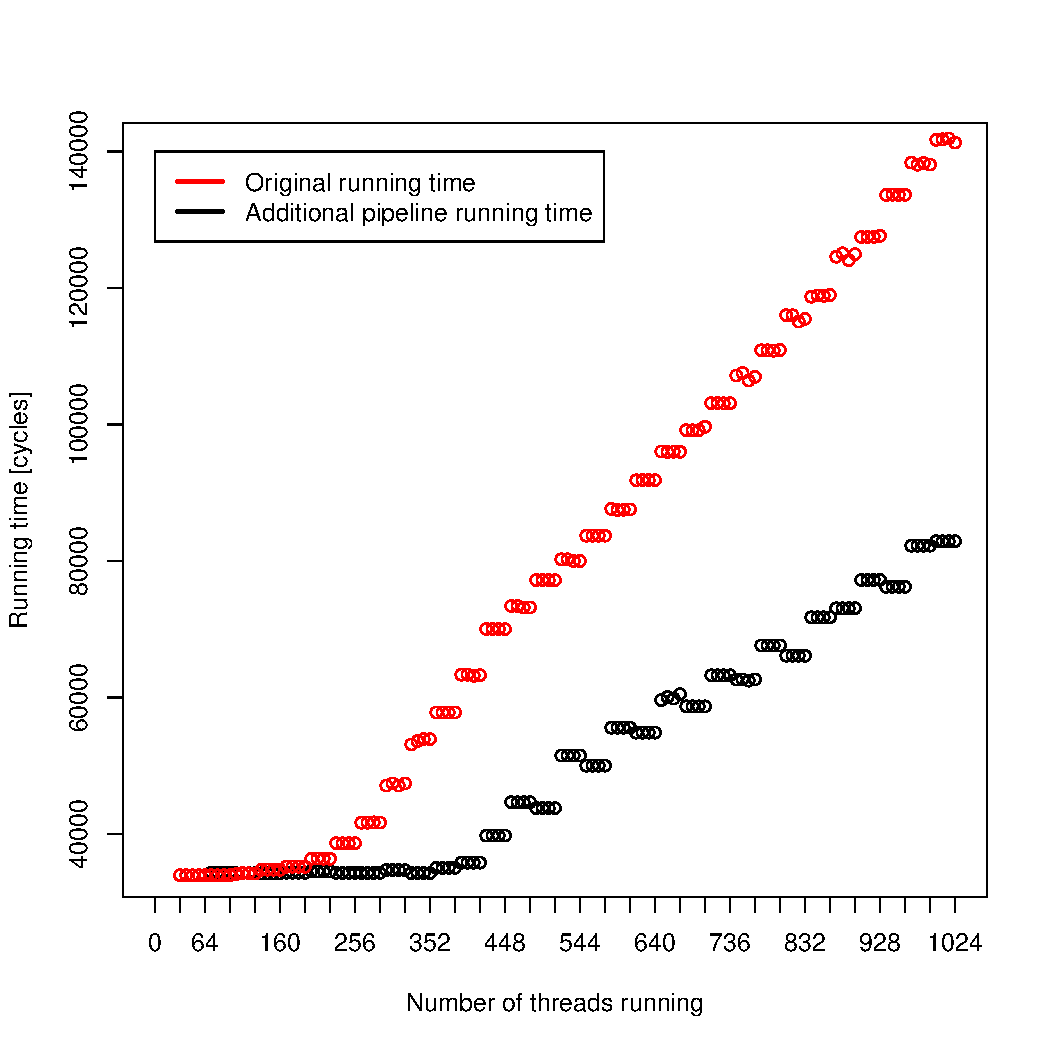
\includegraphics[width=0.9\linewidth]{graphics/improvement-graph}
        \captionsetup{justification=centering}
        \caption{Running times on the default pipeline and on the improved architecture.}
        \label{fig:time_improvement}
    \end{figure}
    
    With higher occupancy, the improved architecture runs the multiplication benchmark in 58\% of the original time.

   \section{Estimated cost variance}
   In order to estimate the cost change, a 24-bit and a 32-bit multipliers have been synthesized with the $65nm$ library GPSVT, which will have to be adapted as the Fermi's architecture is manufactured in $40nm$~\cite{GTX580Datasheet}:
   \[\text{24-bit multiplier} = mul_{24} = 10,354 \mu m^2 \text{ (in $65nm$)} \Rightarrow 6,471 \mu m^2 \text{ (in $40nm$)}.\]
   \[\text{32-bit multiplier} = mul_{32} = 24,052 \mu m^2 \text{ (in $65nm$)} \Rightarrow 14,801 \mu m^2 \text{ (in $40nm$)}.\]
   The size of Fermi's component is also needed and for that a high resolution picture of the chip (Figure ~\ref{fig:fermiChip}) is used in addition to the known total die size which is $520 mm^2$~\cite{G5xxwiki}.
   \begin{figure}[H]
    \centering
        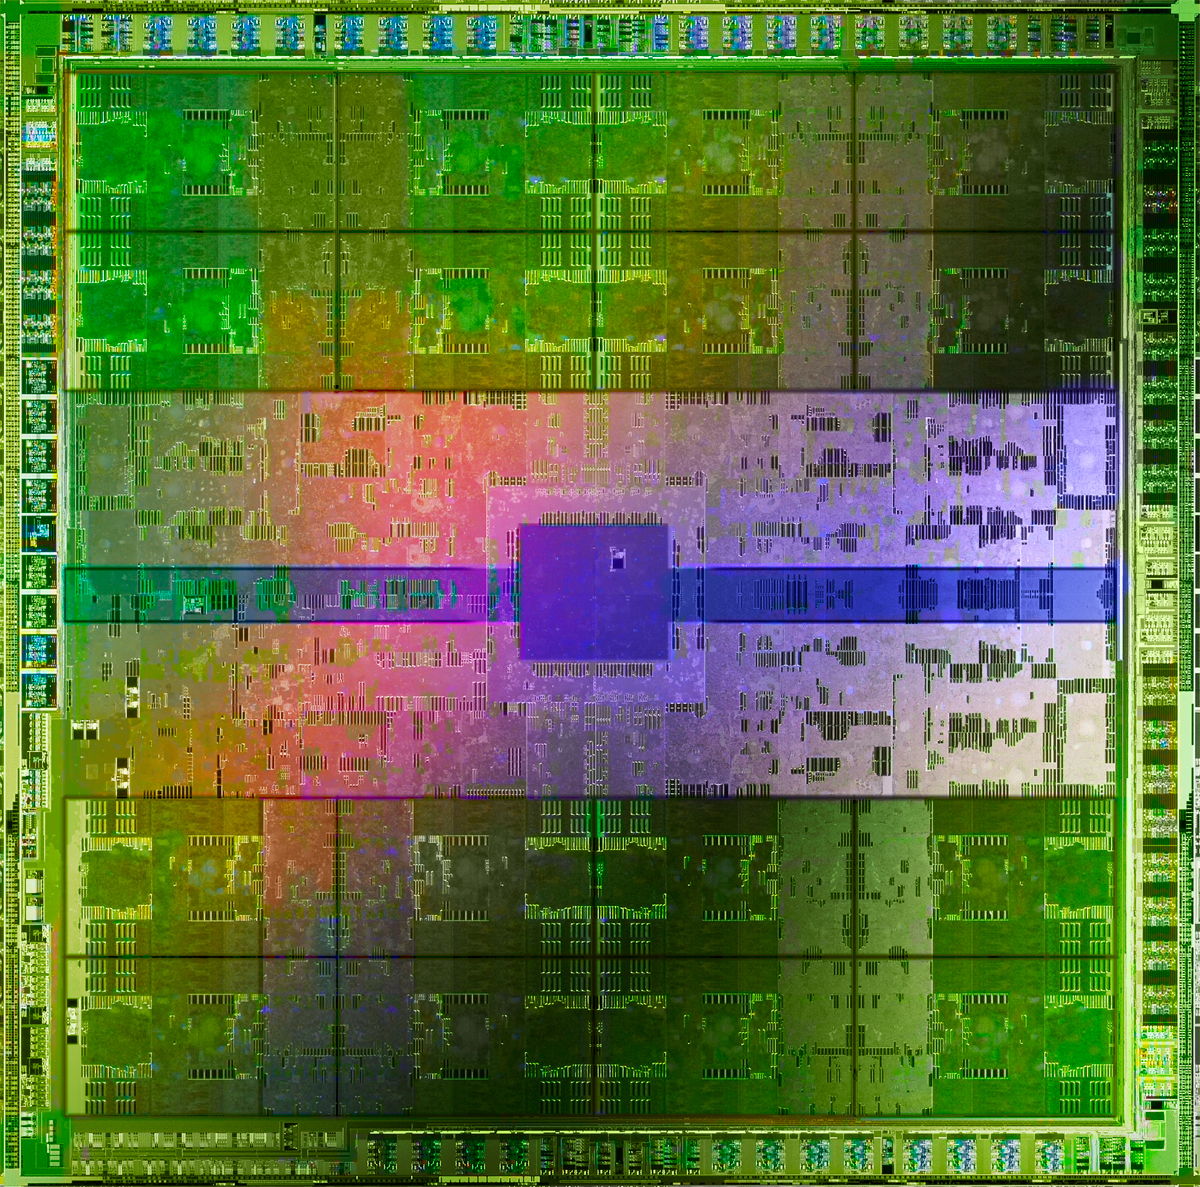
\includegraphics[width=0.7\linewidth]{pictures/FermiChip}
        \captionsetup{justification=centering}
        \caption{Picture of the full GTX580's chip.}
        \label{fig:fermiChip}
    \end{figure}
   
   \subsection{Plan A: 32-bit integer multiplier for every core}
   First thing is to find out the size of a single CUDA core. To do so, the full chip picture (Figure~\ref{fig:fermiChip}) has been analyzed pixel by pixel with its original size of $1200p \times 1200p$ where Figure ~\ref{fig:fermiChipWithLeg} brings out the different part of the chip that were identified and used. Then it was put 
   in correspondance to the known $520mm^2$ area of the full chip and the Table~\ref{tab:sizeChart} has then been filled.
   \begin{figure}[H]
    \centering
        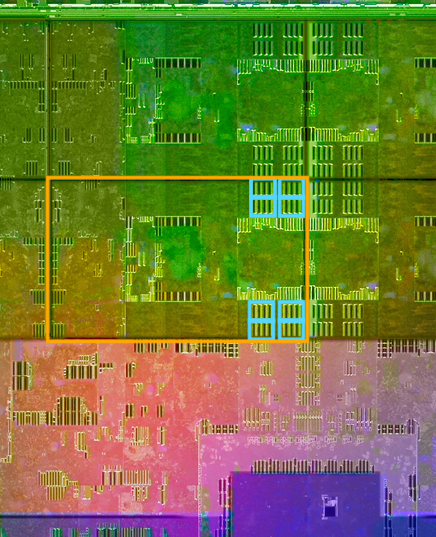
\includegraphics[width=0.7\linewidth]{pictures/FermiChipWithLegend}
        \captionsetup{justification=centering}
        \caption{Inside the orange frame is an SM; inside the blue frame are the 32 CUDA cores of that SM.}
        \label{fig:fermiChipWithLeg}
    \end{figure}
   \begin{figure}[H]
    \centering
        \begin{tabular}{ | l | r | r | }
    	    \hline
    	    Component & Size in $\mu m^2$ & Size in $px^2$ \\ \hline
    	    Full chip &  $5.20 \times 10^8$ & 1,440,000 \\
            Streaming multiprocessor (SM) & $1.50 \times 10^7$ & 41,600 \\
            32 CUDA cores & $9.71 \times 10^5$ & 2688 \\
            Average CUDA core & $3.03 \times 10^4$ &  84 \\ \hline
  	    \end{tabular}
  	\captionsetup{justification=centering}
  	\caption{Size chart between pixels ($px$) and $\mu m^2$ of Fermi's elements.}
  	\label{tab:sizeChart}
    \end{figure}
    
    The size, in the chart, for a single CUA core is an average of a ``float unit and 32-bit multiplier"
    and a ``float unit" CUDA core, in order to find the new core size only half a 32-bit multiplier has to be added.
    \[\text{new core size} = \text{average CUDA core size} + \cfrac{mul_{32}}{2} = 3.77 \times 10^4 \mu m^2 .\] 
    
    Thus, the changes would lead to a size increase of $24.4\%$ of the average core size.
    
    The new SM size can be computed by adding 16 times the 32-bit multiplier cost (once for each cores that doesn't have one already.)
    \[\text{new SM size} = \text{SM size} + mul_{32} \times 16 = 1.53 \times 10^6 \mu m^2 .\]
    Which represents an increase of $1.5\%$ of a SM size.
    
    And eventually, the new size for the whole chip equals 16 times the difference between the old and the new SM size.
    \[\text{new chip size} = \text{full chip size} + (\text{new SM size} - \text{old SM size}) \times 16 =\]
    \[\text{full chip size} + (mul_{32} \times 16) \times  16 = 5.24 \times 10^8 \mu m^2 .\]
    Which represents an increase of $0.73\%$ of the full chip size.
   
   \subsection{Plan B: Every core with only integer support}
   Here the task is to remove the float unit/ float and integer fused unit and replace it with an integer only unit.
   
   In this section $u(\text{FP}_{24})$ represents the CUDA core size that possesses a float unit with only a 24-bit multiplier; $u(\text{FP}_{24}\text{INT}_{32})$ represents the CUDA core size that possesses a float and integer fused unit with a 32-bit multiplier; $u(\text{INT}_{32})$ represents the CUDA core size that only possesses a integer unit with a 32-bit multiplier.
   It is known that:
   \[\
   16u(\text{FP}_{24}) + 16u(\text{FP}_{24}\text{INT}_{32}) = \text{32 CUDA core size} = 9.71 \times 10^5 \mu m^2. \]
   With the previous equation it is found that:
   \[u(\text{FP}_{24}\text{INT}_{32})  =  6.07 \times 10^4 \mu m^2 - u(\text{FP}_{24}).\]
   By an approximation it can be determined that: \[\text{FP}_{24} = mul_{24} * 120\% = 0.78 \times 10^4  \mu m^2.\]
   And then: \[\text{FP}_{24}\text{INT}_{32} = \text{FP}_{24} - mul_{24} + mul_{32} = 1.61 \times 10^4 \mu m^2.\]
   The size of the different CUDA cores should be relative to their units, it follows that:
   \[\alpha = \cfrac{u(\text{FP}_{24})}{\text{FP}_{24}} = \cfrac{u(\text{FP}_{24}\text{INT}_{32})}{\text{FP}_{24}\text{INT}_{32}}.\]
   As the value of $u(\text{FP}_{24}\text{INT}_{32})$ in function of $u(\text{FP}_{24})$ is known. It is found that:
   \[ u(\text{FP}_{24}) = 1.97 \times 10^4 \mu m^2 \text{ and, more interestingly : } \alpha = 2.52.\]
   And finally, it is possible to find the size of the new CUDA core size for plan B:
   \[ \text{new CUDA core size} = u(\text{INT}_{32}) = \alpha \times \text{INT}_{32} = 3.73 \times 10^4 \mu m^2.\]
   Which in this case would represent a $22.9\%$ increase for the size of a CUDA core.
   The new SM size can be computed by adding 16 times the 32-bit multiplier cost (once for each cores which doesn't have one already.)
    \[\text{new SM size} = \text{SM size} + (\text{average CUDA core size} - u(\text{INT}_{32})) \times 16 = 1.51 \times 10^6 \mu m^2. \]
    Which represents an increase of $0.74\%$ of a SM size.
    
    And eventually, the new size of the whole chip is 16 times the difference between the old and the new SM size.
    \[\text{new chip size} = \text{full chip size} + (\text{new SM size} - \text{SM size}) \times 16 =\]
    \[\text{full chip size} + ((\text{average CUDA core size} - u(\text{INT}_{32})) \times 16) \times  16 = 5.22 \times 10^8 \mu m^2. \]
    Which represents an increase of $0.34\%$ of the full chip size.
   
\chapter{Conclusion}
    In this project it has been made obvious that the integer performances 
    (and a fortiori the crypto performances) of Nvidia GPUs are due to an intentional 
    economy on integer hardware but that spares little area for a consequent drop in performances. 
    
    While GPU cards have a computation model well adapted to cryptology, it seems that Nvidia
    cares less and less about integer performances, the integer multiplication throughput
    compared to the number of cores dropped in Kepler compared to Fermi and is even translated as
    multiple instructions in Maxwell~\cite{cudaprog}.
   
    Nvidia's policy to keep everything closed source and secret made the original 
    goal of the project (designing a crypto-specific architecture based on Nvidia GPUs architectures)
    impossible to attain and forced the realization of micro-benchmarking 
    in order to find more information on the architecture we have chosen to base our work on. We went 
    from an initial plan of designing our own many-cores crypto processor to trying to 
    reverse-engineer the work of a full team of engineers.

  \appendix 
 
\chapter{Benchmarking program}
    This code sample is the typical code that was run for an experiment. There were variations on the operations
    inside the for loop (type, numbers of operations) and some experiments were also run without the for loop
    and just the operations.
   
   \lstinputlisting[language=C, breaklines=true]{"integer_multiplication_benchmark.cu"} 

\chapter{Additional benchmarking data}
    \section{Graphics intersteps data}
    The following tables describe the steps between running times in the graphics presented previously. Analyzing them may allow to deduce properties of: 
    \begin{itemize} 
        \item the cores' pipelines, if it represents the delay between dependencies checks;
        \item the scheduling mechanism, if it represents the delaying of threads operations in favor of the launch of other threads.
    \end{itemize}
    
    \centering
    \begin{tabular}{ccc}
\# & Time delta & Ratio of base execution time\\
1 & 1992038 & 0.110518 \\
2 & 2972214 & 0.164899 \\
3 & 1012084 & 0.056151 \\
4 & 2577818 & 0.143018 \\
5 & 1422160 & 0.078902 \\
6 & 2256334 & 0.125182 \\
7 & 1743568 & 0.096733 \\
8 & 2016076 & 0.111852 \\
9 & 1984078 & 0.110077 \\
10 & 2024116 & 0.112298 \\
11 & 1978718 & 0.109779 \\
12 & 2943966 & 0.163331 \\
13 & 1065326 & 0.059104 \\
14 & 2011174 & 0.111580 \\
15 & 1982664 & 0.109998 \\
16 & 2537828 & 0.140799 \\
17 & 1468682 & 0.081483 \\
18 & 2005218 & 0.111250 \\
19 & 1985786 & 0.110172 \\
20 & 2256680 & 0.125201 \\
21 & 1750700 & 0.097129 \\
22 & 2007560 & 0.111380 \\
23 & 1985942 & 0.110180 \\
\end{tabular}

    \begin{table}
\centering
\begin{tabular}{rcc}
\# & Time delta & Ratio of base execution time\\
\hline
1 & 2147856 & 0.119163 \\
2 & 1934380 & 0.107320 \\
3 & 1997060 & 0.110797 \\
4 & 2026158 & 0.112411 \\
5 & 2009622 & 0.111494 \\
6 & 2007910 & 0.111399 \\
7 & 2018118 & 0.111965 \\
\end{tabular}
\caption{Intersteps between single-precision floating-point multiplications benchmarking}
\end{table}

    \pagebreak

    \section{Integer multiplication: 1024 threads starting times}
    \begin{figure}[H]
    		\centering
	    	\includegraphics[width=\scalingfactor\linewidth]{"graphics/starting_times_ratio31"}
	    	\vspace{-15pt}
	    	\captionsetup{justification=centering}    
	    	\caption{Order in which thread batches are started.}
    \end{figure}

\chapter{GPGPU-Sim faithfulness}
    To make sure GPGPU-Sim was usable with the benchmarks used in this project, the basic benchmarks were
    ran on the GTX 580 and on GPGPU-Sim with its default GTX 480 configuration (in which the only difference
    between the GTX 580 and GTX 480 is the number of SMs). The benchmark we have run are:
    \begin{itemize}
        \item Float multiplication benchmark;
        \item Integer multiplication benchmark;
        \item Float matrix multiplication; 
        \item Integer matrix multiplication.
    \end{itemize}

    The running times yielded are plotted in Figure~\ref{fig:gpu-sim-corr}.
    \begin{figure}[H]
    \centering
        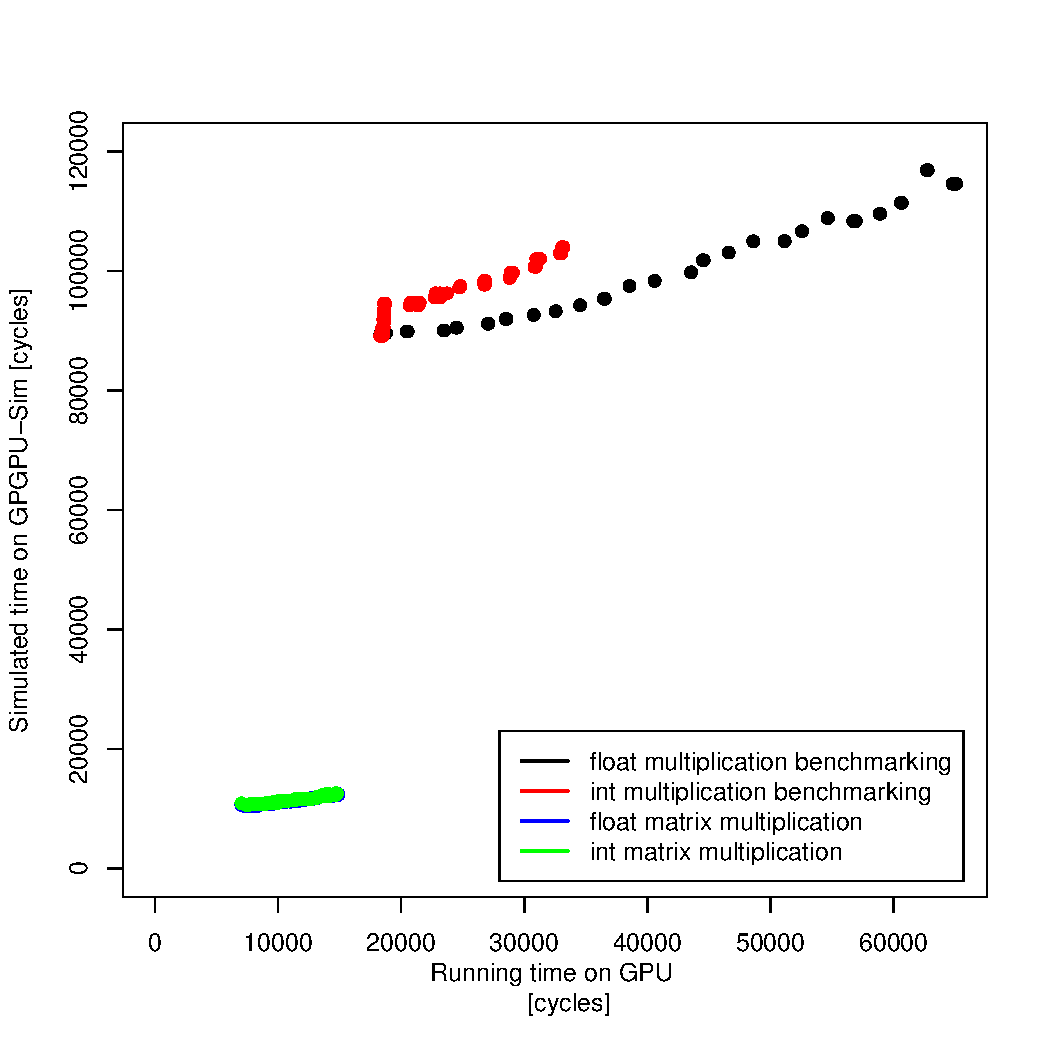
\includegraphics[width=0.9\linewidth]{graphics/comparative_graph}
        \captionsetup{justification=centering}
        \caption{Running times on the GTX 580 plotted against GPGPU-Sim running times.}
        \label{fig:gpu-sim-corr}
    \end{figure}

    The Pearson's correlation for each experiments are in Table~\ref{tab:gpu-sim-corr}.
    \begin{figure}[H]
    \centering
        \begin{tabular}{ | r | c | }
    	    \hline
    	    Benchmark type & Running times correlation \\ \hline
    	    Float multiplication benchmark & 94\% \\
            Integer multiplication benchmark & 98\% \\
            Float matrix multiplication & 98\% \\
            Integer matrix multiplication & 97\% \\ \hline
  	    \end{tabular}
  	\captionsetup{justification=centering}
  	\caption{Correlation between GPU running times and GPGPU-Sim simulated times.}
  	\label{tab:gpu-sim-corr}
    \end{figure}

    While GPGPU-Sim has a higher clock count than the GTX 580 and its evolution is quite different, the running times are still strongly correlated.
   
   \bibliography{project_report}{}
   \bibliographystyle{plain}


\end{document}
